% The Stationary paper.  Every number is recomputed from run data or exact solutions:
% see VERIFICATION.md (paper value, recomputed value, how).  \pending{} marks numbers that wait for
% the reruns listed there; NOTES.md lists the open items.
% Target: Phys. Rev. D (REVTeX 4.2).  For Class. Quantum Grav. switch to the iopart class.
\documentclass[aps,prd,twocolumn,superscriptaddress,nofootinbib,floatfix]{revtex4-2}
\usepackage{amsmath,amssymb,bm}
\usepackage{graphicx}
\usepackage{booktabs}
\usepackage{xcolor}
\usepackage[colorlinks=true,linkcolor=blue,citecolor=blue,urlcolor=blue]{hyperref}

\newcommand{\todo}[1]{\textcolor{red}{[TODO: #1]}}
\newcommand{\pending}[1]{\textcolor{blue}{[#1]}}
\newcommand{\dd}{\mathrm{d}}
\newcommand{\Ric}{\mathrm{Ric}}

\begin{document}

\title{Solving the static Einstein equations with physics-informed neural networks}

\author{\todo{authors}}
\affiliation{\todo{affiliations}}

\date{\today}

\begin{abstract}
A classical existence theory guarantees that the stationary vacuum Einstein equations, posed in
the region outside a ball, have a unique solution for boundary data close enough to flat space,
depending continuously on the data. We present a physics-informed neural network (PINN) solver
for this boundary-value problem in the static case. The unknowns are a Riemannian 3-metric $h$ and
the squared norm $\lambda$ of the static Killing vector, in harmonic gauge; the data are
$\lambda$ and the induced metric on an inner sphere, and asymptotic flatness is imposed by Robin
conditions on an outer sphere. The connection is the Christoffel symbol of the network metric.
We test the solver on Schwarzschild in harmonic coordinates and on two-rod Weyl solutions, on the
symmetry axis and rotated so that no symmetry is left. For quadrupolar data, which have no
closed-form solution, we compare with an independent spectral solution of the same problem. The
harmonic gauge and the inner data leave the asymptotic chart free to translate, and this
translation dominates the error until it is fixed by Cederbaum's pseudo-Newtonian centre of mass,
a conserved flux of the static equations; with it, the solution agrees with the spectral one to
five to six orders below the size of the perturbation. Finally, we read the Geroch--Hansen mass
moments of the computed solutions off the symmetry axis, without constructing Weyl coordinates;
they reproduce the exact moments of the Weyl solutions and the reference moments of the
quadrupolar one.
\end{abstract}

\maketitle

% =====================================================================================
\section{Introduction}
% =====================================================================================

For many years there has been a mathematical theory of the stationary Einstein equations in an
asymptotic region of spacetime, namely the region outside a ball~\cite{Reula1989}. It states that
boundary data close enough to those of flat spacetime, together with the asymptotic conditions,
produce a unique solution that depends continuously on the data. Very few attempts have been made
to explore this theory numerically~\cite{TODO_numerics_stationary}. Here we show that this is
possible, and that it opens a new window on these spacetimes.

The method also gives a simple way to explore other systems of possible physical importance:
systems in which one solves for a Riemannian metric together with other fields, through equations
that contain its Ricci tensor. Examples are the construction of minimal-energy data
sets~\cite{TODO_minimal_energy} and the equations that give higher-order Newtonian-limit
expansions~\cite{TODO_newtonian_limit}. \todo{more examples}

We restrict this work to the static Einstein equations. The stationary case is no harder from the
point of view of the approximation method, and is left for a continuation of this work.

Physics-informed neural networks~\cite{Raissi2019} represent the unknown fields by a neural network
and minimise the squared residual of the equations and boundary conditions over sampled points.
They need no mesh, handle the non-compact exterior through a logarithmic radial variable, and treat
a configuration with no symmetry exactly as they treat a symmetric one. A small residual does not
by itself mean a small error, so every result below is graded against an exact solution or an
independent reference.

Section~\ref{sec:equations} states the equations, the gauge, the boundary and asymptotic conditions,
and the residual gauge freedom. Section~\ref{sec:code} describes the solver. Section~\ref{sec:tests}
tests it on exact solutions, Sec.~\ref{sec:quadrupole} solves the quadrupolar problem, and
Sec.~\ref{sec:moments} extracts the multipole moments. Appendix~\ref{app:repro} lists what is
needed to repeat every computation.

% =====================================================================================
\section{The static Einstein equations}\label{sec:equations}
% =====================================================================================

\subsection{Variables and field equations}

We write a static vacuum spacetime as
\begin{equation}
  g = -\lambda\,\dd t^2 + \lambda^{-1} h ,
  \label{eq:lineelement}
\end{equation}
where $h$ is a Riemannian metric on the spatial slice and $\lambda = -\xi\cdot\xi$ is the squared
norm of the static Killing vector $\xi = \partial_t$; if $g = -N^2\dd t^2+\gamma$, then
$\lambda = N^2$ and $h = N^2\gamma$. The vacuum equations become
\begin{align}
  R_{ab}(h) &= \frac{1}{2\lambda^{2}}\,\nabla_a\lambda\,\nabla_b\lambda, \label{eq:ricci}\\
  h^{ab}\nabla_a\nabla_b\lambda &= \frac{1}{\lambda}\,h^{ab}\nabla_a\lambda\nabla_b\lambda . \label{eq:lam}
\end{align}
With $U = \tfrac12\ln\lambda$ these read $\Ric(h) = 2\,\dd U\otimes\dd U$ and $\Delta_h U = 0$.

\subsection{Gauge}

We impose harmonic coordinates on $h$,
\begin{equation}
  \Gamma^i \equiv h^{jk}\Gamma^i{}_{jk} = S^i ,
  \label{eq:gauge}
\end{equation}
with $S^i = 0$; equivalently $\Delta_h x^i = 0$ for the Cartesian-like coordinates
$x^i = \rho\, n^i$. For the Weyl tests we instead use a source built from the candidate's own
metric,
\begin{equation}
  S^i = (h_{\rho\rho} - 1)\, h^{ij}\partial_j \ln \rho_n , \qquad
  \rho_n = \bigl|x - (x\cdot n)\,n\bigr| ,
  \label{eq:cylsource}
\end{equation}
with $n$ the symmetry axis, which Weyl's canonical form
$h = e^{2k}(\dd\rho^2+\dd z^2)+\rho^2\dd\phi^2$ satisfies exactly.

\subsection{The exact spherical family}

In the harmonic chart the spherically symmetric solutions are
\begin{equation}
  h_{ij} = \Bigl(1-\frac{R_0^2}{\rho^2}\Bigr)\delta_{ij} + \frac{R_0^2}{\rho^2}\,n_in_j , \qquad
  \lambda = k\,\frac{\rho-R_0}{\rho+R_0} ,
  \label{eq:schw}
\end{equation}
i.e.\ $h = \dd\rho^2+(\rho^2-R_0^2)\,\dd\Omega^2$. With $k=1$ this is Schwarzschild in harmonic
coordinates: $M = R_0$, areal radius $r = \rho+R_0$, $\lambda = 1-2M/r$. The harmonic condition
still allows the radial maps $\rho\to c_1\rho + c_2 F_2(\rho)$,
$F_2 = 2R_0+\rho\ln\frac{\rho-R_0}{\rho+R_0}$, fixed by the round inner metric and $h\to\delta$.

\subsection{Boundary and asymptotic conditions}\label{sec:bcs}

The domain is the shell $\rho_{\rm in}\le\rho\le\rho_{\rm out}$.

\paragraph{Inner sphere.} We prescribe $\lambda$ and the induced metric,
\begin{equation}
  \lambda = \lambda_0 + S_1\, n\cdot e + S_2\, P_2(n\cdot e), \qquad
  P h P = \frac{r_{\rm in}^2}{\rho_{\rm in}^2}\, P ,
  \label{eq:innerbc}
\end{equation}
with $P = I - n\otimes n$, $r_{\rm in}$ the areal radius of the sphere in $h$ and $e$ the data
axis. The components $h_{rr}$ and $h_{rA}$ are not data: in harmonic gauge the $l\ge1$ sectors
have exactly as many decaying solutions as~\eqref{eq:innerbc} imposes conditions, and one more
condition (e.g.\ $h_{rA}=0$) leaves no decaying solution. $\lambda_0$ is chosen so that
$\lambda\to1$ on the spherical branch.

\paragraph{Outer sphere.} Asymptotic flatness is imposed by Robin conditions of order $n$,
\begin{equation}
  B_n[f] \equiv \prod_{i=0}^{n-1}\bigl(\rho\,\partial_\rho + p_f + i\bigr)\,(f-f_\infty) = 0 ,
  \label{eq:robin}
\end{equation}
which annihilate the decaying powers $\rho^{-p_f},\dots,\rho^{-p_f-n+1}$. The exponents follow from
the equations, $\delta h\sim\rho^{-2}$, $\Gamma\sim\rho^{-3}$, $\lambda-1\sim\rho^{-1}$; the exact
solution~\eqref{eq:schw} gives local decay rates $2.00$, $3.005$ and $0.952$ at $\rho=20$. For
the scalar we impose the condition on the Geroch--Hansen potential~\cite{Geroch1970,Hansen1974}
\begin{equation}
  \mathcal P = \frac{1-\lambda^2}{4\lambda} = -\tfrac12\sinh 2U ,
  \label{eq:Ppot}
\end{equation}
whose monopole $M/\rho + M^3/(3\rho^3)+\dots$ has no $\rho^{-2}$ term, unlike
$\lambda = 1-2M/\rho+2M^2/\rho^2-\dots$. The same conditions are imposed on a few spheres inside
$\rho_{\rm out}$ (at $0.7$, $0.8$, $0.9\,\rho_{\rm out}$): they hold at every radius for the exact
solution, and a single sphere can be satisfied by a thin boundary layer. For the quadrupolar
problem we add spherical means of order-one Robin combinations at $\rho_{\rm out}$,
$\langle(\rho\partial_\rho+3)(h_{rr}-1)\rangle$, $\langle(\rho\partial_\rho+2)(g_2-1)\rangle$ with
$g_2 = \tfrac12(\operatorname{tr}h - h_{rr})$, and $\langle(\rho\partial_\rho+1)\mathcal P\rangle$;
without them $h$ drifts towards a multiple of the identity. On $\lambda$ itself such a pin would
be violated by the exact solution, by $-6.59\times10^{-5}$ at $\rho_{\rm out}=100$ (a loss floor
of $4.3\times10^{-7}$); on $\mathcal P$ the floor is $1.5\times10^{-11}$. $\lambda_\infty=1$ is
fixed.

\subsection{The residual gauge freedom and the centre of mass}\label{sec:gaugefreedom}

The harmonic condition fixes the chart only up to harmonic diffeomorphisms $x\to x+\xi$,
$\Delta_h\xi = 0$. One of them is left free by our data: $\xi = 0$ on the inner sphere and
$\xi\to a$ at infinity. It keeps the chart harmonic and the inner data unchanged, and translates
the asymptotic chart by $a$. Its effect on the scalar, $\xi\cdot\nabla\lambda$, vanishes at
$\rho_{\rm in}$ and decays like $\rho^{-2}$, so the outer conditions barely penalise it: for
$|a|\approx0.04$ it changes the dipole of $\mathcal P$ at $\rho=100$ by $\approx2.5\times10^{-6}$.

It is fixed by the centre of mass. Since $U$ and the coordinates $x^i$ are both $h$-harmonic,
Green's identity makes
\begin{equation}
  D^i(S) = \oint_S\bigl(x^i\,\partial_\nu U - U\,\partial_\nu x^i\bigr)\,\dd A_h
  \label{eq:comflux}
\end{equation}
the same on every closed surface $S$ enclosing the inner sphere, and $D = 4\pi M a$ for a mass $M$
displaced by $a$. This is the pseudo-Newtonian centre of mass that Cederbaum introduced for static
(``geometrostatic'') isolated systems~\cite{Cederbaum2012}, written in our variables. It is
quasi-local, obeys an addition theorem for several separated sources, coincides with the ADM and
constant-mean-curvature centres of mass in suitable asymptotic coordinates, and converges to the
Newtonian centre of mass in the Newtonian limit~\cite{Cederbaum2012,CederbaumNerz2015}. The
asymptotic notions it is compared with go back to Regge--Teitelboim and
Beig--\'O~Murchadha~\cite{ReggeTeitelboim1974,BeigOMurchadha1987} and to the foliation-based
definitions of Huisken--Yau, Metzger, Huang, Corvino--Wu and
Eichmair--Metzger~\cite{HuiskenYau1996,Metzger2007,Huang2009,Huang2010,CorvinoWu2008,EichmairMetzger2012}
(see Ref.~\cite{CorvinoPollack2011}); Cederbaum's analysis builds on the asymptotics of static
fields of Beig, Beig--Simon and Kennefick--\'O~Murchadha~\cite{Beig1980,BeigSimon1980,KennefickOMurchadha1995}.
We impose $d \equiv D/4\pi = 0$ on a set of spheres. This is a gauge choice, available for any
data; Sec.~\ref{sec:quadrupole} shows that without it the translation mode is the largest error
of the computed solution.

% =====================================================================================
\section{The solver}\label{sec:code}
% =====================================================================================

\paragraph{Networks.} The inputs are $n = x/\rho$ and
$t = \ln(\rho/\rho_{\rm in})/\ln(\rho_{\rm out}/\rho_{\rm in})\in[0,1]$, optionally with
$\rho_{\rm in}/\rho$; the body is a $\tanh$ multilayer perceptron, the output layer is initialised
small so that training starts near flat space. The network outputs $h$ and $\lambda=e^u$, and the
connection is the Christoffel symbol of $h$, computed by automatic differentiation, so the
compatibility equation holds identically. (A first-order variant outputs $\Gamma$ as well and adds
compatibility as a residual; on the same Schwarzschild problem it is three orders of magnitude
less accurate, Sec.~\ref{sec:schw}, and it must never be trained with a vanishing compatibility
weight, which the code refuses.) For axisymmetric problems
\begin{gather}
  h_{ij} = (1+a)\,\delta_{ij} + b\, n_in_j + \tfrac{c}{2}\,(n_iz_j+z_in_j) + d\, z_iz_j ,
  \nonumber\\
  \lambda = e^{u} ,
  \label{eq:axisym}
\end{gather}
with $a,b,c,d,u$ functions of $(t,\mu=n\cdot z)$: 2285 parameters at width 20 and depth 6 with the
decay feature (2265 without). The general three-dimensional network of the same size has 2347.
Spherically symmetric tests use $h = \alpha(\rho)\delta+\beta(\rho)nn$.

\paragraph{Loss.} With $R_g$ the residual of group $g$ (Ricci, gauge, scalar equation), the loss is
\begin{multline}
  L = \sum_g w_g\,\overline{(\rho^{p_g}R_g)^2}
     + w_{\rm in}\overline{r_{\rm in}^2} + w_{\rm out}\overline{r_{\rm out}^2} \\
     + w_{\rm pin}\sum\langle r\rangle^2 + w_{\rm com}\sum_S|d|^2 ,
  \label{eq:loss}
\end{multline}
with means over the sampled points. $p=(2,1,2)$ makes every residual dimensionless; for the
quadrupolar problem we use $p=(4,3,4)$, an extra weight $\rho^4$ that determines the far field.
$w_{\rm in}=w_{\rm out}=w_{\rm pin}=w_{\rm com}=100$ (10 for the Weyl tests). The centre-of-mass
term uses a fixed quadrature on each sphere (24 Gauss--Legendre nodes in $\mu$ times 8 in $\phi$).
Interior points are drawn log-uniformly in $\rho$ with uniform directions and redrawn every 500
iterations; every result is checked on fresh samples, where the loss agrees with the training
loss to within \pending{a few per cent}.

\paragraph{Training.} Adam~\cite{KingmaBa2014} for 5000 steps, then the self-scaled Broyden
quasi-Newton method SSBroyden~\cite{Urban2025SSBroyden,TODO_crunch} with a dense inverse Hessian
carried between blocks of 250 iterations, an Armijo line search (up to 100 trials) and
scale-invariant curvature guards, in stages of 10000 iterations. \pending{If round P confirms it:
no other optimiser is needed.} Everything runs in double precision with JAX~\cite{jax2018} on
NVIDIA A30 GPUs; one value and gradient at 16384 points costs 0.048~s.

\paragraph{A spectral reference.}\label{sec:specref} For the quadrupolar problem we built an
independent solution: the spherical background~\eqref{eq:schw} plus an axisymmetric,
reflection-even perturbation, with Legendre modes $l\le10$ in the angle and 36 Chebyshev modes in
$\ln\rho$ for each of the five metric functions and $\lambda$ (1008 unknowns), solved by
Gauss--Newton on exactly the residual vector of the loss~\eqref{eq:loss}. Its loss is
$2.8\times10^{-11}$, its $l=2$ tail decays as $\rho^{-3.00}$ from $\rho=20$ to 100, and evaluated
with a network run's own loss on that run's samples it gives $2.8\times10^{-11}$ as well: it is a
solution of the same discrete problem, obtained by an unrelated method. Its rotated version grades
the off-axis runs.

% =====================================================================================
\section{Tests with exact solutions}\label{sec:tests}
% =====================================================================================

\subsection{The pipeline on exact solutions}

The exact solution~\eqref{eq:schw}, packed exactly as a network packs its outputs, gives a total
loss below $10^{-16}$. The two-rod Weyl solution gives $1.3\times10^{-28}$ with the source
\eqref{eq:cylsource}; with $S=0$ it does not, because the Weyl chart is not harmonic
($|\Gamma^i|$ up to $9.2\times10^{-3}$ on the sphere $\rho=7.5$). The rotated Weyl solution
solves the system to $3\times10^{-14}$ or better at every residual. (The averaged pins of
Sec.~\ref{sec:bcs} are designed for the quadrupolar problem and are not satisfied by these
solutions, at the $10^{-9}$ level; the tests run without them.)

\subsection{Schwarzschild in harmonic coordinates}\label{sec:schw}

The spherical network with $R_0=1$, $\lambda_0 = 0.381966$ on the sphere of $h$-areal radius 2 and
Robin conditions at $\rho_{\rm out}=100$ recovers the exact family. Table~\ref{tab:firstorder}
compares the metric-only and first-order formulations on the problem with a manufactured Robin
source: the first-order network finds the same geometry in a different harmonic chart, with
$h_{rr}$ off by tens of per cent, because the compatibility residual is nearly flat along this
gauge mode; deriving $\Gamma$ from $h$ removes it. With the homogeneous Robin conditions (no
source), the metric-only network gives \pending{max errors of the rerun} against the exact solution.

\begin{table}
\caption{First-order against metric-only network on the same Schwarzschild problem (manufactured
Robin source, $\rho_{\rm out}=100$, 20000 Adam + 2000 SSBroyden iterations). \pending{values of
the reruns; the original runs gave the numbers shown}.}
\label{tab:firstorder}
\begin{ruledtabular}
\begin{tabular}{lcc}
 & first order ($h,\Gamma,\lambda$) & metric only ($h,\lambda$) \\
\hline
final loss & $6.3\times10^{-6}$ & $5.8\times10^{-8}$ \\
$\max|\delta h|$ & $3.3\times10^{-1}$ & $5.3\times10^{-5}$ \\
$\max|\delta\Gamma|$ & $1.7\times10^{-1}$ & $2.3\times10^{-4}$ \\
$\max|\delta\lambda|$ & $1.3\times10^{-2}$ & $2.9\times10^{-5}$ \\
\end{tabular}
\end{ruledtabular}
\end{table}

\subsection{Weyl two-rod solutions}

The Weyl class~\cite{Weyl1917} gives exact static axisymmetric solutions with nontrivial
multipoles. We use two rods, $U_{\rm rod} = \tfrac12\ln[(R_a+R_b-L)/(R_a+R_b+L)]$ (mass $L/2$
each) with $k$ by quadrature; the inner data and the Robin sources are taken from the exact
solution and the gauge is~\eqref{eq:cylsource}. For two equal rods (masses 1, gap 1) on the shell
$[7.5,75]$ the axisymmetric network trained with SSBroyden from a random initialisation reaches a
loss of $2.06\times10^{-13}$ in 3000 iterations, with maximum errors $6.7\times10^{-7}$ in $h$ and
$9.0\times10^{-8}$ in $\lambda$ (Fig.~\ref{fig:weyl}). Unequal rods (masses 1 and 0.1) give
$2.4\times10^{-14}$, $3.4\times10^{-7}$ and $5.2\times10^{-8}$. Their moments are in
Sec.~\ref{sec:moments}. Moving the inner sphere towards the rods raises the curvature on it by
four orders of magnitude, and the error with it (Table~\ref{tab:weylclose}).

\begin{table}
\caption{Weyl rods (masses 1 and 0.1), inner sphere moved towards the rods; 3000 SSBroyden
iterations, standard units.}
\label{tab:weylclose}
\begin{ruledtabular}
\begin{tabular}{lcccc}
shell & dist.\ to horizon & $R_{ab}R^{ab}(\rho_{\rm in})$ & $\max|\delta h|$ & loss \\
\hline
$[7.5,75]$ & 5.0 & $3.3\times10^{-6}$ & $3.4\times10^{-7}$ & $2.4\times10^{-14}$ \\
$[4,40]$ & 1.5 & $5.8\times10^{-3}$ & $1.5\times10^{-5}$ & $7.1\times10^{-13}$ \\
$[3.5,35]$ & 1.0 & $5.3\times10^{-2}$ & $7.3\times10^{-5}$ & $3.1\times10^{-12}$ \\
\end{tabular}
\end{ruledtabular}
\end{table}

\begin{figure}
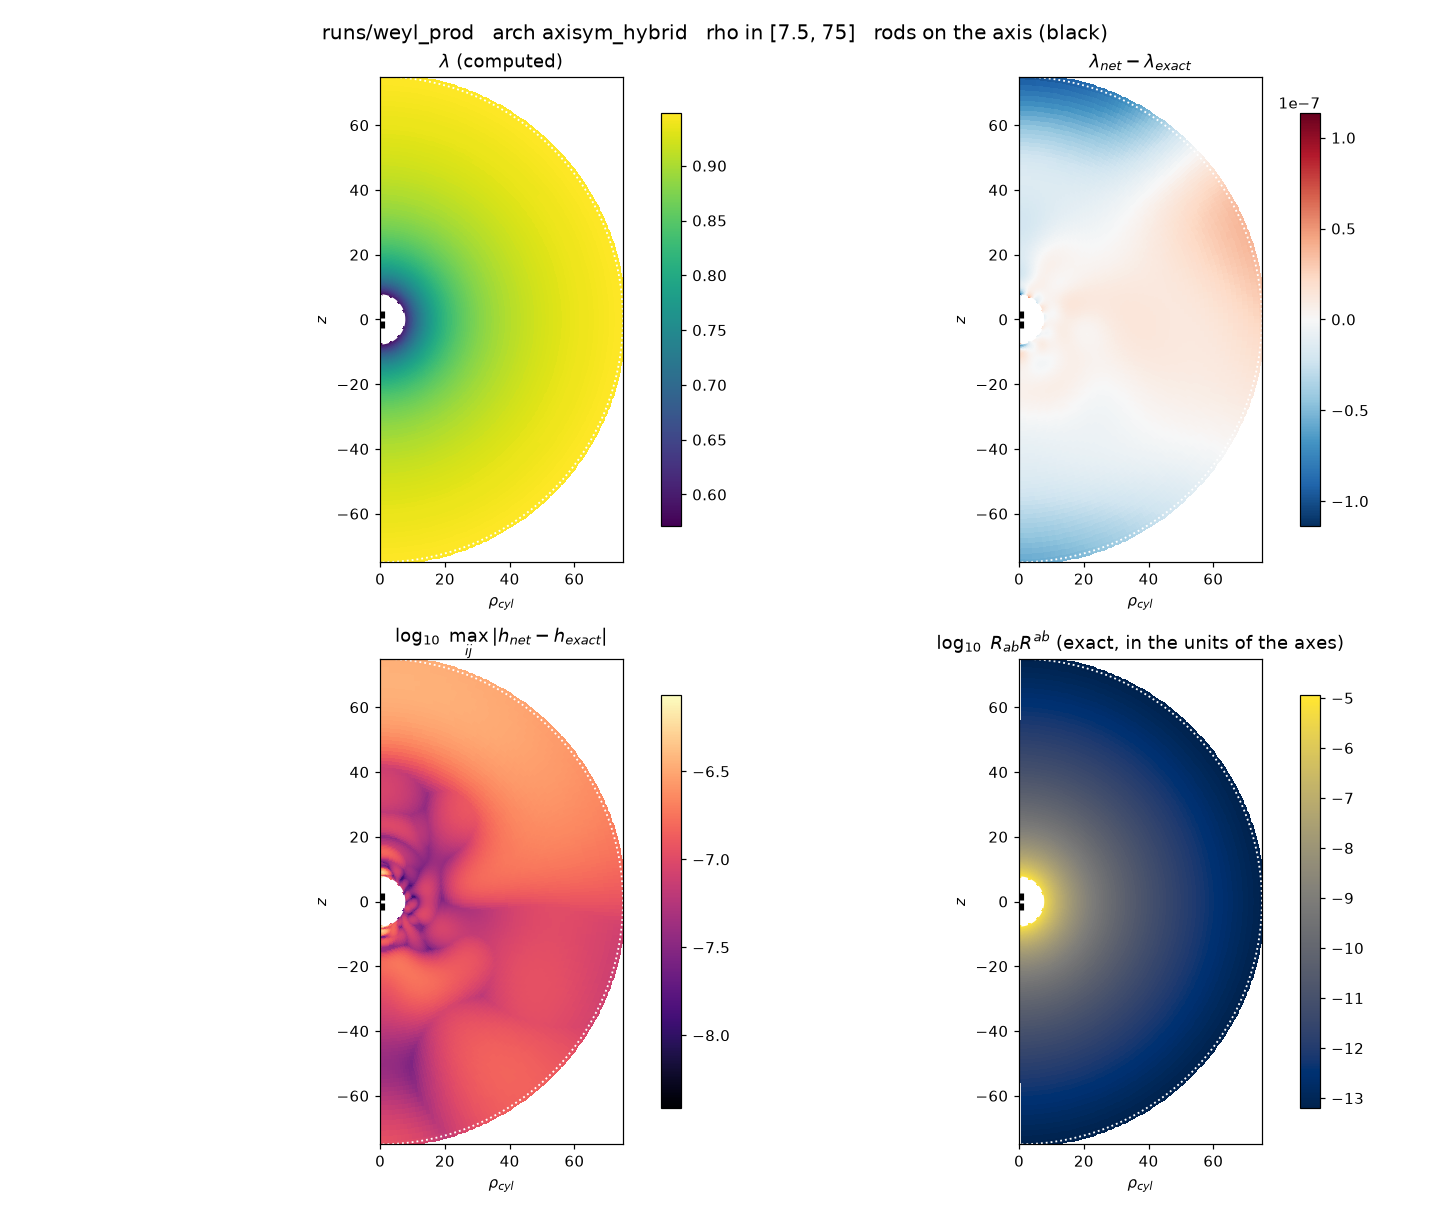
\includegraphics[width=\columnwidth]{figs/weyl_plane.png}
\caption{Equal-mass Weyl rods on the shell $[7.5,75]$ (meridional plane): computed $\lambda$;
$\lambda_{\rm net}-\lambda_{\rm exact}$; $\log_{10}\max_{ij}|h_{\rm net}-h_{\rm exact}|$;
$\log_{10}R_{ab}R^{ab}$ of the exact solution. \todo{regenerate without the internal title}}
\label{fig:weyl}
\end{figure}

\subsection{A rotated Weyl configuration}

Rotating the closest configuration by $45^\circ$ removes every symmetry. The equations are
covariant, so the rotated fields are again a solution, but the gauge is a statement about a chart
and the source~\eqref{eq:cylsource} must be taken about the rotated axis $n = R\hat z$; in
harmonic gauge the rotated solution has a residual of $2.6\times10^{-2}$. The general
three-dimensional metric-only network, with 8192 collocation points, reaches \pending{loss, max
errors of weyl\_rot45\_hyb}. In this problem the number of collocation points mattered more than
the number of iterations: an earlier first-order run on 2048 points lowered its mean-square loss
by a factor 8 ($1.75\times10^{-4}\to2.28\times10^{-5}$) over 6500 further iterations while every error grew, the residual concentrating on
a few points; with four times the points the errors fell with the loss.

% =====================================================================================
\section{Quadrupolar data}\label{sec:quadrupole}
% =====================================================================================

\subsection{The problem}

We take $R_0 = 1/\sqrt3$, the inner sphere $\rho_{\rm in}=1$ with $r_{\rm in}=1$ (so
$\lambda_0 = 1/3$), $\rho_{\rm out}=100$, and
\begin{equation}
  \lambda|_{\rho_{\rm in}} = \tfrac13 - \tfrac1{12}\,P_2(\cos\theta) ,
\end{equation}
a 25\% perturbation of the spherical value, with no known closed-form solution. Linear theory
predicts a pure $l=2$ response decaying like $\rho^{-3}$, no $l=1$ part and an $l=0$ back-reaction
of order $S_2^2$. Against the spherical solution the perturbation has an rms size of
$2.0\times10^{-2}$ in $\lambda$ and $2.2\times10^{-2}$ in $h$ near the inner sphere, and
$2.6\times10^{-4}$ and $3.5\times10^{-6}$ for $30<\rho<100$. We grade against the spectral
reference.

\subsection{Without and with the centre-of-mass condition}

Two runs with identical commands, except for the centre-of-mass term
(Appendix~\ref{app:repro}), show what the condition does (Table~\ref{tab:com},
Fig.~\ref{fig:com}). Without it, the error near the inner sphere is of order \pending{$10^{-3}$},
and it is odd under $z\to-z$ (modes $l=1,3$), which the even data forbid; every term of the loss
is exactly reflection symmetric, so nothing forces this part: it is the translation mode of
Sec.~\ref{sec:gaugefreedom}. The flux~\eqref{eq:comflux} is constant in $\rho$ but nonzero,
\pending{$d_z$}, and far out the solution is the reference translated by $a = d/M$. With
$d = 0$ imposed on the spheres $\rho = 1, 1.5, 3, 10, 30, 100$, the error falls by
\pending{four to five} orders of magnitude, to \pending{five to six} orders below the size of the
perturbation, and the loss to \pending{the level of the reference}.

\begin{table*}
\caption{Error against the spectral reference (angular rms) by radial region, for the same run
without and with the centre-of-mass condition. \pending{values of qp\_nocom and qp\_com}.}
\label{tab:com}
\begin{ruledtabular}
\begin{tabular}{lccccccccc}
 & loss & \multicolumn{4}{c}{$\lambda$ error} & \multicolumn{4}{c}{$h$ error} \\
 & & 1--3 & 3--10 & 10--30 & 30--100 & 1--3 & 3--10 & 10--30 & 30--100 \\
\hline
perturbation size & & $2.0\times10^{-2}$ & $2.5\times10^{-3}$ & $7.6\times10^{-4}$ & $2.6\times10^{-4}$ & $2.2\times10^{-2}$ & $4.5\times10^{-4}$ & $3.1\times10^{-5}$ & $3.5\times10^{-6}$ \\
without centre of mass & \pending{} & \pending{} & & & & & & & \\
with centre of mass & \pending{} & \pending{} & & & & & & & \\
\end{tabular}
\end{ruledtabular}
\end{table*}

\begin{figure*}
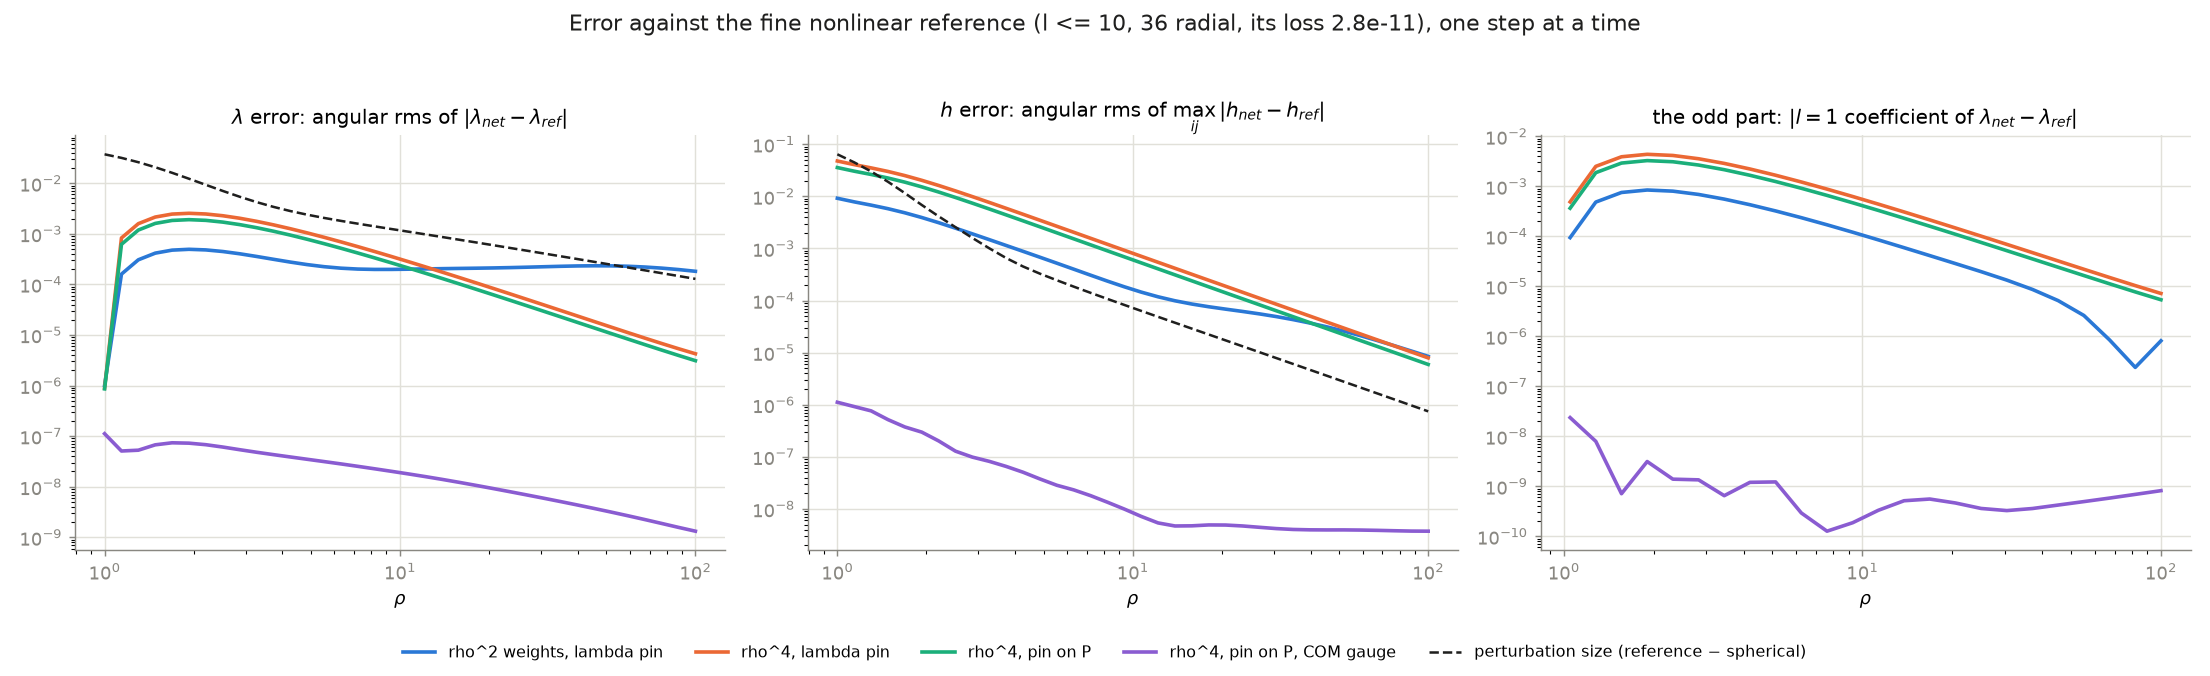
\includegraphics[width=\textwidth]{figs/com_steps.png}
\caption{Error against the spectral reference without and with the centre-of-mass condition:
angular rms of $\lambda_{\rm net}-\lambda_{\rm ref}$, of $\max_{ij}|h_{\rm net}-h_{\rm ref}|$, and the
$l=1$ coefficient of $\lambda_{\rm net}-\lambda_{\rm ref}$. Dashed: the perturbation (reference minus
spherical solution). \pending{regenerate for qp\_nocom and qp\_com}}
\label{fig:com}
\end{figure*}

\subsection{Off-axis data}

The same datum about the axis $(1,0,1)/\sqrt2$ is a fully three-dimensional problem whose solution
is the rotated axisymmetric one. With the general metric-only network the error against the
rotated reference is \pending{qp\_rot: rms $\lambda$, $h$}, i.e.\ \pending{N and M} times below the
perturbation. The same network on the unrotated datum gives the same errors after the same
budget, so the rotation itself costs nothing; the general ansatz reaches a loss
\pending{three to four} orders above the axisymmetric one, the error concentrating in $h$ near the
inner sphere.

% =====================================================================================
\section{Multipole moments}\label{sec:moments}
% =====================================================================================

\paragraph{Extraction from the axis.} For a static axisymmetric vacuum solution the
Geroch--Hansen moments~\cite{Geroch1970,Hansen1974,Beig2000} follow from the potential on the
symmetry axis in canonical Weyl coordinates,
$g = -e^{2U}\dd t^2+e^{-2U}[e^{2k}(\dd W^2+\dd Z^2)+W^2\dd\phi^2]$: with the static Ernst potential
$\xi = -\tanh U$ on the axis, $\xi(0,Z) = \sum_j m_j/|Z|^{j+1}$, the moments are $M_j = m_j$ for
$j\le3$ and $M_4 = m_4 - \tfrac17 m_0(m_0m_2-m_1^2)$~\cite{SotiriouApostolatos2004}; equivalently,
from $U(0,Z) = \sum_r U^{(r)}/|Z|^{r+1}$, $M_0=-U^{(0)}$, $M_1=-U^{(1)}$,
$M_2 = \tfrac13(U^{(0)})^3-U^{(2)}$, $M_3=(U^{(0)})^2U^{(1)}-U^{(3)}$~\cite{FHP1989}. Weyl coordinates
need not be built, because only the axis is used: in our variables $U = \tfrac12\ln\lambda$ and
$W = |\partial_\phi|_h$; on the part of the axis that reaches infinity $k=0$, so there $\dd Z$ is the
proper $h$-length along the axis; the inner ball cuts the axis in two, and the offset between the
branches is the change of $Z$ along a meridian semicircle, $\dd Z = \star\dd W$ in the meridian
metric. We fit $\xi$ on both branches and fix the origin of $Z$ by mass centring ($M_1=0$); the
error bar is the spread over fit windows starting at $1$--$1.5\,\rho_{\rm in}$ and fit orders 6 and
8. On exact solutions this returns: Schwarzschild in harmonic coordinates, $M_0=R_0$ to
$10^{-12}$ and $M_l$ below $10^{-11}$ for $1\le l\le4$; the equal Weyl rods, $M_0 = 2$ and
$M_2 = 2.500000$; the unequal rods, the closed-form moments to $10^{-5}$ relative and the centre of
mass $z=1.309091$; Curzon, $M_2 = -M^3/3$ and $M_4 = 19M^5/105$, although $U$ itself has no
quadrupole.

\paragraph{The Weyl networks.} The trained solutions give $M_0 = 2.000001$ and $M_2 = 2.49950$ for
the equal rods (exact 2 and 2.5), and $M_0 = 1.100000$, $M_2 = 0.29105$, $M_3 = -0.5016$ with the
centre of mass at $z = 1.3091$ for the unequal rods (exact 1.1, 0.290909, $-0.49983$, 1.309091).
\pending{rotated Weyl, metric-only network}.

\paragraph{The quadrupolar solution.} Table~\ref{tab:moments} lists the moments. The data raise the
mass from the background value $R_0 = 0.57735$ to $M_0 = 0.583847$, a nonlinear back-reaction of
1.1\% in the monopole, and the quadrupole moment is $M_2 = 0.1747$. The run without the
centre-of-mass condition, whose pointwise error is \pending{$10^{-3}$}, has moments within
\pending{$10^{-5}$} of the reference: moments are geometric, and the translation mode moves the
chart, not the geometry. The extraction shows the mode directly: the centre of mass of that run,
measured from the centre of the coordinate sphere of radius $\rho$, \pending{grows from $\sim0$ at
$\rho=1$ to the translation $a$ far out}, while with the condition it is \pending{$\sim10^{-7}$} at
every radius.

\begin{table}
\caption{Geroch--Hansen moments of the quadrupolar solution: the spectral reference, and the
differences network $-$ reference with the same fit windows (the reference's window spread,
$1.2\times10^{-4}$ in $M_2$ and $7\times10^{-4}$ in $M_4$, largely cancels in the differences).
\pending{rows for qp\_com, qp\_nocom, qp\_rot}.}
\label{tab:moments}
\begin{ruledtabular}
\begin{tabular}{lccc}
 & $M_0$ & $M_2$ & $M_4$ \\
\hline
reference & $0.583847$ & $0.17471$ & $0.0220$ \\
with centre of mass & \pending{} & & \\
without centre of mass & \pending{} & & \\
3-D network, rotated data & \pending{} & & \\
\end{tabular}
\end{ruledtabular}
\end{table}

\paragraph{Decay of the multipoles.} Expanding $\mathcal P$ in Legendre modes $c_l(\rho)$ about the
solution's own axis, the local power $\dd\ln|c_l|/\dd\ln\rho$ of the reference is $-1.00$, $-3.00$
and $-5.0$ for $l=0,2,4$ (the last out to $\rho\approx30$, where $c_4\sim10^{-10}$), and its odd
modes are at $10^{-16}$. \pending{The same for qp\_com and qp\_rot.} In the mass-centred harmonic
chart $c_l\rho^{l+1}$ tends to $0.58387$, $0.1747$ and $0.0220$, i.e.\ to $M_0$, $M_2$ and $M_4$,
consistently with harmonic coordinates being asymptotically Cartesian and mass
centred~\cite{Thorne1980,Gursel1983}: a second, independent route to the same numbers.

% =====================================================================================
\section{Conclusions}\label{sec:conclusions}
% =====================================================================================

A PINN solves the exterior boundary-value problem of the static vacuum Einstein equations with
prescribed inner data and asymptotic flatness, and reproduces exact solutions with and without
symmetry. Two ingredients are essential: a network whose connection is derived from its metric,
and a complete gauge fixing. Harmonic coordinates and the inner data leave the asymptotic chart
free to translate; the mode is invisible to every residual except at a very low level, and it is
the largest error until the pseudo-Newtonian centre of mass is fixed. We expect the same issue, and
the same remedy, in any elliptic formulation of the stationary problem whose inner data do not fix
the asymptotic frame. The Geroch--Hansen moments of the computed solutions can be read off the
symmetry axis without constructing Weyl coordinates, and they are insensitive to that translation.
The extension to the stationary equations is the natural next step.

\appendix
\section{Reproducing the results}\label{app:repro}

\todo{repository URL and the commit the paper's numbers come from.} The code is the
\texttt{Stationary} package of that repository: \texttt{stationary/train.py} (the solver; every
option below is a flag of \texttt{python -m stationary.train}), \texttt{stationary/specref.py}
(the spectral reference), \texttt{stationary/gh\_moments.py} (the moments). Software: Python 3.14,
JAX 0.11.1, Flax 0.12.9, Optax 0.2.8, in double precision (\texttt{JAX\_ENABLE\_X64=1}); hardware:
NVIDIA A30 (24~GB). Each result is produced by the commands below, all in the repository.
\begin{itemize}
\item Exact-solution checks: \texttt{tests/test\_pipeline.py}, \texttt{verify\_weyl.py},
  \texttt{tests/test\_gh\_moments.py}.
\item Schwarzschild tests (Table~\ref{tab:firstorder}): \texttt{Paper/commands\_schwarzschild.sh}.
\item Weyl tests: the configurations stored with each run (\texttt{runs/weyl\_*/config.json});
  the rotated test, \texttt{Paper/commands\_weyl.sh}.
\item Quadrupolar data: \texttt{recipe\_pq16k.sh} (the problem) and the stages
  \texttt{qp\_com\_*}, \texttt{qp\_nocom\_*}, \texttt{qp\_rot\_*} of \texttt{mendieta\_submit.sh}
  \pending{wall times}.
\item The spectral reference: \texttt{python -m stationary.specref} \pending{exact command of the
  fine reference}.
\item Grading and moments: \texttt{scripts/grade\_rotated.py}, \texttt{scripts/fresh\_sample\_loss.py},
  \texttt{scripts/gh\_moments\_runs.py}, \texttt{scripts/tail\_decay.py}.
\end{itemize}

\begin{acknowledgments}
We thank the Palma group \todo{names} for the Crunch implementation of SSBroyden, and the CCAD of
the Universidad Nacional de C\'ordoba for computing time on Mendieta and its JupyterHub.
\todo{funding}. The initial setting and the exact-solution tests were done with the help of
DeepSeek; the quadrupole runs and the centre-of-mass fix were done with Claude (Anthropic).
\end{acknowledgments}

\bibliography{refs}

\end{document}
